\documentclass[a4paper, 11pt, titlepage]{article}
\usepackage{fancyhdr}
\usepackage{graphicx}
\usepackage{imakeidx}
\usepackage{makeidx}
\usepackage{mathtools}
\usepackage[spanish]{babel}
\usepackage{listings}

\title{\textbf{Enrutamiento Cebolla \& Tor}}
\author{Francisco Javier Balón Aguilar}
\date{Diciembre de 2018}

\renewcommand{\figurename}{Imagen}

\begin{document}

\maketitle
\renewcommand{\contentsname}{Índice}
\tableofcontents
\newpage

\section{Breve contextualización histórica y conceptual}

    Tor son las siglas de \emph{The Onion Routing}, algo que podríamos traducir al español como <<enrutamiento cebolla>> 
    por su criptografía a capas, como veremos más adelante. Se trata de un proyecto de software libre creado originalmente 
    con fines militares por parte del ejército y la inteligencia norteamericanas de comunicaciones seguras, privadas y 
    anónimas entre espías y agentes en campo enemigo orientado a las operaciones realizadas en territorios principalmente 
    soviéticos.

    Tor consiste en una gran red descentralizada compuesta por nodos repartidos por todo el mundo, a través de los cuales 
    viajan nuestros paquetes de red ofreciéndonos anonimato. Tras ser abandonado por el ejército fue reciclado por la 
    \emph{Electronic Frontier Foundation}\footnote{Organización sin ánimo de lucro con sede en San Francisco, Estados 
    Unidos con el objetivo declarado de dedicar sus esfuerzos a conservar los derechos de libertad de expresión en la era 
    de las comunicaciones.} y, finalmente soportado por su propia comunidad.

    El objetivo de Tor es preservar la privacidad y el anonimato (diferenciados, más adelante ahondaremos en sus diferencias 
    y similitudes) de los que navegan por Internet, manteniendo comunicaciones seguras, asegurando la integridad de la 
    información, pretendiendo evitar monitorización y registro de actividad, etc. Con el fin de proteger la \emph{libertad}
    \footnote{Entendiendo esta libertad como un libre albedrío digital, sin entrar a valorar definiciones filosóficas, 
    pues no es el caso de este estudio.} de los usuarios en Internet y evitar la censura.

    Actualmente Tor es utilizado por diversos perfiles, desde disidentes políticos de diversos países, denunciantes, 
    periodistas, gobiernos, hackers --tanto de sombrero blanco como de sombrero negro--, vendedores de diversa índole 
    e, incluso narcotraficantes, delincuentes, etc. Este punto será desglosado más tarde.

    \subsection{Deep web o red profunda \& Darknet o red oscura}

        Es necesario continuar esta contextualización definiendo la red profunda de la que tanto se habla y con tan poco 
        fundamento en muchas ocasiones. La definición es clara y concisa: <<La deep web es el contenido de internet que 
        \emph{no está indexado} por los motores de búsqueda convencionales, debido a diversos factores.>> Como podemos 
        ver, no existe delincuencia ni malicia en la propia definición de esta. Un servidor privado conectado mediante 
        \emph{Dynamic DNS}\footnote{Técnica de traducción de nombres de dominio (\emph{DNS}) que permite trabajar con 
        direcciones IP dinámicas.} de un particular o cualquier base de datos empresarial (que lógicamente no es accesible
        mediante indexadores) podría considerarse y, de hecho, se considera parte de la red profunda.

        Cuando la cultura popular se refiere a la red Tor como homóloga a la Deep Web, lo hace erróneamente. Sí es cierto 
        que debemos admitir a la red Tor (y cualquier red semejante o parecida, como las redes \emph{i2p} o \emph{freenet}) 
        como parte de la deep web. Para solucionar este conflicto de conceptos, se ideó la conocida como \emph{darknet} o 
        \emph{red oscura}, haciéndo referencia exclusivamente a estas redes <<especiales>>; concepto que vuelve a ser 
        salpicado por la <<leyenda negra>> que lo absorve --que no exime de la existencia de inmoralidad y delincuencia 
        en ella, hay que admitir--.

        Por ello, en el presente documento se hablará \emph{con propiedad} a la hora de mencionar la \emph{deep web} y 
        la \emph{darknet}.

    \subsection{Privacidad y anonimato}
            
        Ya conocemos el funcionamiento de Tor, ¿pero qué usos prácticos tiene respecto a la privacidad y el anonimato?, 
        ¿conocemos la diferencia entre privacidad y anonimato?. Es necesario primero, como en toda ciencia, definir los 
        conceptos con los que vamos a tratar, ya que a menudo se utilizan igual erróneamente.

        Si observamos la segunda definición otorgada por la \emph{Real Academia Española} sobre la \textbf{privacidad}, 
        <<Ámbito de la vida privada que se tiene derecho a proteger de cualquier intromisión>> y la contraponemos a la 
        definición de \textbf{anonimato} --concretamente la quinta definición de anónimo--: <<Situación de quien oculta 
        su nombre>>, podemos observar una correlación clarísima en cuanto al ocultamiento o protección. Ambos conceptos 
        protegen algo. Pero el objeto protegido cambia con cada definición:
        
        En un caso normal, una personalidad realiza una determinada acción:

        \begin{quote}
            \center <<\textit{Juan está comiendo patatas}>>.
        \end{quote}

        La \textbf{privacidad} protege las acciones que la personalidad realiza. Se sabe que \emph{Juan} está haciendo 
        \emph{algo}, pero no sabemos qué.

        \begin{quote}
            \center <<\textit{¿Qué está haciendo Juan?}>>.
        \end{quote}

        El \textbf{anonimato} protege a la personalidad que realiza la acción. Sabemos que \emph{alguien} está 
        \emph{comiendo patatas}, pero no sabemos quién.
        
        \begin{quote}
            \center <<\textit{¿Quién está comiendo patatas?}>>.
        \end{quote}

        Como podemos ver, depende también de la posición del observador y, de esta forma podremos combinarlas para ganar 
        tanto privacidad como anonimato. 
        La red Tor tiene como objetivo dotar a sus usuarios de ambas capacidades, logrando en mayor o menor medida el 
        deseado:

        \begin{quote}
            \center <<\textit{¿Quién está haciendo qué?}>>.
        \end{quote}

\section{Técnica teórica}

    Es necesario comenzar, pues con la técnica de la red Tor. A priori puede parecer muy complejo, pero en lo que avanza 
    el desarrollo de este documento podremos comprobar que su funcionamiento es sencillo; no eximiendo un grandísimo 
    potencial de uso y, como veremos más adelante, un gran margen de mejora. 

    \begin{figure}[htp]
        \centering
        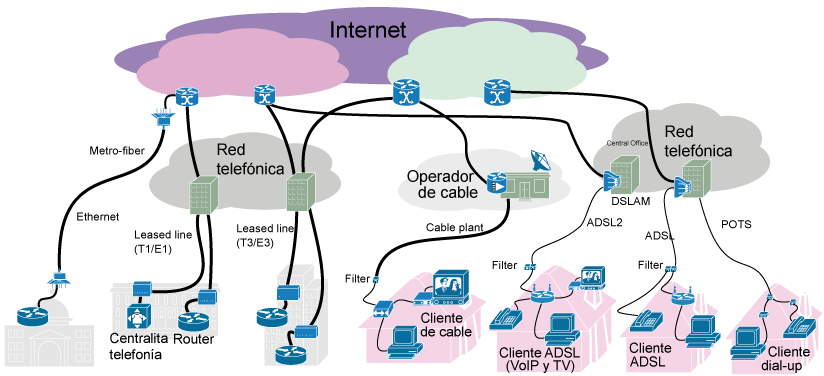
\includegraphics[width=0.9\textwidth]{resources/esquemaInternet.png}
        \caption{Esquema básico del funcionamiento de Internet}
        \label{fig:esquema}
    \end{figure}
        
    Si nos conectamos a Internet de manera habitual, nuestra dirección IP pública y un conjunto de información más quedará 
    expuesta, tanto para el destino de la conexión como para \emph{hombres en el medio}\footnote{\emph{Man in the Middle} 
    es una conocida técnica de espionaje y manipulación de paquetes en red}, como pueden ser hackers, \emph{sniffers}, las 
    propias empresas que nos proveen servicios, autoridades, gobiernos, etc. Además si la conexión no se encuentra cifrada 
    podrán incluso filtrarse contraseñas y mensajes secretos y confidenciales.

    Todo lo que hacemos en Internet puede ser --y se encuentra, de hecho-- monitorizado y almacenado.
    
    Por contraposición, Tor crea una ruta al azar de nodos distribuidos por el mundo, a través de los cuales viajarán 
    nuestras peticiones, de esta forma el destino de nuestros paquetes no conocerá nuestra dirección IP, sino la del nodo 
    de salida (al igual que usando un \emph{proxy} o una \emph{VPN}), y de la misma forma, el nodo de salida no conocerá 
    la dirección IP del origen, sino del nodo anterior a él en la ruta. A su vez, el nodo de entrada no conocerá el destino 
    de la conexión, simplemente su destino será el segundo nodo. De esta forma se permite alcanzar un alto grado de 
    anonimato, ya que, en el caso de ser vulnerado o amenazado un nodo, nuestra información se mantendrá anónima.
    
    Anteriormente comentamos el origen del nombre de Tor: el enrutador cebolla. Esto se debe a su peculiar forma de usar 
    la criptografía sobre la información que realiza para que proteger la confidencialidad e integridad de la información 
    de los propios servidores, incluso: \emph{cifrado por capas}. Completando la explicación anterior, nuestro cliente de 
    Tor alojado en nuestra máquina calculará al azar la ruta antes mencionada, que en este caso digamos que corresponde a 
    3 nodos para agilizar la explicación, el nodo de entrada en Washington, el segundo nodo en Praga y el nodo de salida 
    en Moscú. Con la ruta ya calculada, cifrara el paquete, digamos, la petición de una simple página HTML con la clave 
    pública del nodo de salida, posteriormente volverá a cifrar el paquete ya cifrado con la clave pública del segundo nodo 
    y, finalmente, con la clave del nodo de entrada y, una vez terminado el cifrado por capas, será enviado al nodo de 
    entrada, donde usará su clave privada para descifrarlo y lo reenviará al segundo nodo, que hará lo mismo.
    
    \begin{figure}[htp]
        \centering
        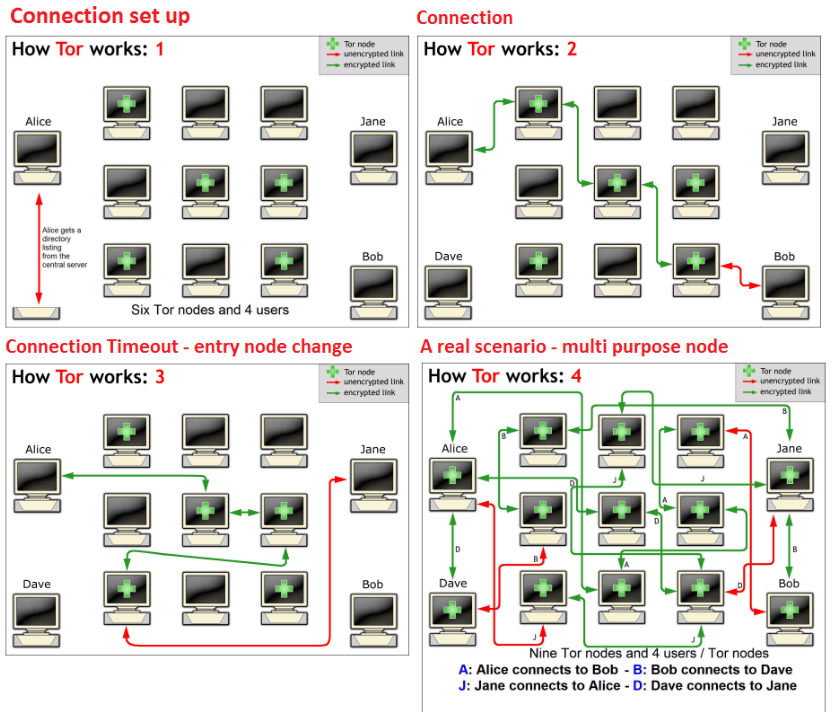
\includegraphics[width=0.9\textwidth]{resources/torconn.png}
        \caption{Representación de los diferentes pasos para la efectuación de una conexión en Tor}
        \label{}
    \end{figure}
        
    El proceso continuará hasta llegar al nodo de salida y este (Moscú) pedirá la página deseada (recordamos que esta 
    página verá como cliente a Moscú y no a nosotros) y realizará el mismo proceso de cifrado pero a la inversa, para 
    devolverla al cliente de Tor. A continuación será deslogaso este tema tan amplio como la criptografía, en concreto 
    lógicamente la de la red que estamos estudiando.

    \subsection{Criptografía}

        Tor es el heredero del sistema desarrollado por el \emph{Departamento de Defensa de Estados Unidos}. Ahondando 
        un poco más en el tema, podemos llamar a David M. Goldshlag, Michael Reed y Paul Syverson los padres del 
        \emph{encaminamiento cebolla} o \emph{onion routing}, idea algorítmica que precede y, es a su vez, núcleo del 
        concepto y de la técnica de Tor.

        \begin{figure}[htp]
            \centering
            
\includegraphics[scale=1.00]{resources/davidchaum.jpg}
            \caption{David Chaum (1955) inventor de protocolos criptográficos}
            \label{chaum}
        \end{figure}

        David M. Goldshlag, Michael Reed y Paul Syverson se basaron y aplicaron las ideas de \emph{redes de mezclado} 
        de David Chaum (Figura \ref{chaum}). El objetivo fundamental y sin añadidos de estos conceptos criptográficos 
        no es más que permitir \textbf{infraestructuras para comunicaciones privadas sobre redes públicas}.

        Tor no es la única red basada en estos conceptos criptográficos y algorítmicos, pero sí es la más conocida, la 
        más utilizada y, en principio, la que mejor resultados otorgan a los usuarios. Además, el tratarse de una red 
        de software libre y de código abierto ha permitido la afluencia de una gran comunidad de desarrolladores que 
        la han hecho crecer y mejorar. Dicho esto, podemos hacer menciones honoríficas a otras redes que, como Tor, 
        siguen esta idea: \emph{Freedom Network}, \emph{Onion Routing}, \emph{MixMaster}, \emph{Babel}, \emph{Mixminion}, 
        \emph{Zach Brown's Onion}, \emph{PipeNet}, \emph{IronKey}, \emph{MorphMix}, y \emph{Tarzan}.

        \subsubsection{Idea primigenia criptográfica}

            La idea primera era utilizar \emph{criptografía de clave asimétrica tradicional}. Este sistema es vulnerable 
            a ataques basados en \emph{sniffing de tráfico}. Efectivamente, supongamos que un atacante puede \emph{esnifar} 
            todos los datos que son intercambiados entre los nodos. Si finalmente el atacante consigue comprometer todos 
            los routers (accedediendo a sus claves privadas) entonces este puede descifrar todo el tráfico almacenado 
            anteriormente. 

            Para acotar este problema podríamos cambiar periódicamente las claves (pública y privada) de los routers. 
            Para ello estableceríamos un periodo de tiempo a la finalización del cual las claves caducarían y sería 
            necesario establecer nuevas claves. La clave pública habría que difundirla y la antigua clave privada se 
            destruiría para que no pudiera ser obtenida nunca, asegurando así la persistencia de la seguridad del 
            tráfico que se realizó usando la antigua clave. Sería acertado que el cambio de claves fuera frecuente ya 
            que esto limitaría la cantidad de tiempo que tiene A para comprometer B y C, pero a la vez requeriría que 
            los routers del sistema contactaran frecuentemente con un sistema que les actualizara las nuevas claves lo 
            que llevaría a problemas de escalabilidad. En resumidas cuentas: viable pero poco práctico.
        
        \subsubsection{Criptografía de Onion Routing, padre de Tor}

            Onion Routing establece un circuito de claves simétricas, a partir de una criptografía de clave pública 
            mediante una estructura de datos con capas (de ahí la denominación de \emph{cebolla} - \emph{onion} que 
            posteriormente fue reutilizada por nuestro objeto de estudio).

            \begin{figure}[htp]
                \centering
                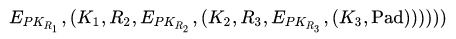
\includegraphics[scale=3.00]{resources/onionroutingcrypto.png}
                \caption{Fórmula matemática que muestra el funcionamiento de Onion Routing en base a 3 saltos o capas.}
                \label{}
            \end{figure}

            $PK_{R i} = Ri$ ; $Ri \in \{R_{1},R_{2},R_{3}\}$ 

            $K_{i}$ = material que permite establecer la/s clave/s de sesión compartida (puede haber una para cada sentido 
            de la comunicación) entre el origen de la comunicación (el iniciador).
            
            \textbf{Observar que la capa final se identifica porque no contiene ni dirección destino, ni datos con 
            significado para ser transmitidos.}

            La principal desventaja de este enfoque es que no provee de \emph{<<perfect forward secrecy>>}. Supongamos que 
            un circuito se construye desde el iniciador con la secuencia de nodos A,B,C y que A es un router malicioso y 
            por tanto el atacante puede descifrar todo lo que pasa y ha pasado por él. Si A graba todo el tráfico y en el 
            último momento se compromete B (el cual sabe quien es el último nodo C), entonces se compromete C y A puede 
            saber con quien se está comunicando el iniciador.

        \subsubsection{Enfoque telescópico}
           
            Y finalmente llegamos a la criptografía utilizada por Tor. Ésta utiliza una construcción \emph{incremental} 
            e \emph{interactiva} del circuito, a la que llaman \emph{enfoque telescópico}.
            
            \begin{figure}[htp]
                \centering
                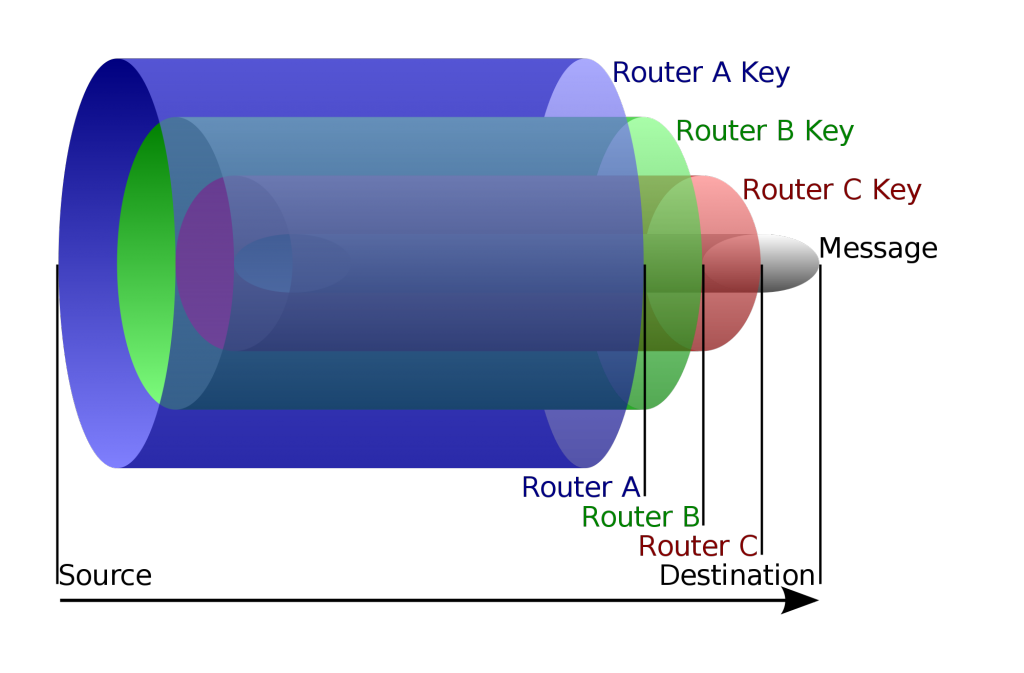
\includegraphics[width=0.7\textwidth]{resources/onion.png}
                \caption{Representación gráfica del cifrado en cebolla}
                \label{}
            \end{figure}

            En concreto Tor se apoya en el Tor Authentication Protocol (siglas TAP), cuya seguridad fue probada en el modelo 
            de <<oráculo aleatorio>>. Tor lo que hace es realizar una ejecución secuencial de múltiples instancias de TAP, 
            estableciendo un circuito de autenticación RSA de un solo sentido (el iniciador no se autentica nunca). Para 
            ello se utiliza el circuito parcialmente construido hasta ese momento. Podemos decir que en cada tramo sucesivo 
            del circuito se realiza una negociación interactiva de claves (\emph{protocolo de establecimiento de claves de 
            Diffie-Hellman}\footnote{Protocolo de establecimiento de claves entre partes que no han tenido contacto previo, 
            utilizando un canal inseguro y de manera anónima (no autentificada).}). 

            En el TAP la clave pública del nodo sólo se utiliza para iniciar la comunicación durante la cual se establece 
            la clave temporal de sesión vía el protocolo de establecimiento de claves de \emph{Diffie-Hellman}. Las claves 
            se forman a partir del intercambio de mensajes en lugar de ser enviadas de forma cifrada. Por tanto, una vez 
            que la sesión finalice (el circuito ha dejado de usarse) y se destruyan las claves de sesión, si se compromete 
            un router (se obtiene su clave privada) esto no permite al adversario recuperar las claves de sesión eliminadas 
            y descifrar así el tráfico cifrado bajo esa clave que pudiera tener almacenada. Por tanto tenemos 
            \emph{\textbf{perfect forward secrecy}}. Por otra parte ya no es necesario almacenar hashes de las estructuras 
            de datos previamente procesadas para evitar ataques de replay. Reinyectando uno de los mensajes del handshake 
            del protocolo de establecimiento de claves de \emph{Diffi-Hellman} provoca unos resultados de clave de sesión 
            diferentes y por tanto ya no sería un ataque efectivo.

    \subsection{Red \emph{inproxy} y \emph{outproxy}}

        Tor permite la salida a Internet utilizando los repetidores que se encuentran dentro de la red. Esto es una solución 
        \emph{outproxy} en donde los usuarios pueden salir hacia Internet utilizando la plataforma de anonimato, los 
        repetidores que se encuentran disponibles en la red. 

        Las redes \emph{inproxy}, por el contrario no permiten esto, solamente permiten la navegación dentro de la red. Es 
        el concepto más puro de una \emph{VPN}\footnote{\emph{Red Privada Virtual} es una tecnología que permite la 
        extracción cifrada y <<tunelada>> de una red de área local (\emph{LAN}) a una red pública.} en donde todos los 
        repetidores se pueden comunicar entre ellos pero no permiten salir de ella.
        
        Por ello podemos concluir en que Tor es una red \emph{inproxy} a la misma vez que es una red \emph{outproxy}; 
        dependiendo del uso que le demos podemos obtener las ventajas de una u otra, o ambas simultáneamente.
    
        \subsubsection{Hidden Services}

            La red Tor no es sólo una red <<proxy>> o red de entrada-salida a Internet. Tor implementa además un protocolo 
            que permite la configuración de servidores dentro de la misma red, sin necesidad de salir de ella (algo que 
            aumenta notoriamente la privacidad y el anonimato, tanto del lado del cliente, como del lado del servidor). 
            Podemos considerarlo quizás, una red privada, una intranet propia de la red. Estos servidores se conocen como 
            \emph{hidden services} (Servicios ocultos, en castellano).
            
            Un \emph{hidden service} es un servidor común, la mayor parte de ellos corriendo sobre \emph{GNU/Linux} y 
            el resto \emph{FreeBSD}, \emph{Unix}, \emph{GNU/Hurd}, etc. En ocasiones incluso podemos encontrar servidores 
            ocultos corriendo sobre \emph{Microsoft Windows Server}, aunque es algo poco común. Estas máquinas ofrecen 
            los mismos servicios que un servidor convencional (web, mail, FTP, etc).
            
            Pero, al contrario de un servidor común, \textbf{el cliente no conoce la dirección IP del mismo}. Los nodos 
            de Tor cumplen la función de servidores DNS, que de mediante intercambio de claves criptográficas obtiene la 
            clave pública que identifica a este servidor dentro de la red de nombres de dominio. Esta clave seguida de la 
            extensión \emph{.onion} como podemos ver en la imagen \ref{onion} constituye el dominio del servidor.
        
            \begin{figure}[htp]
                \centering
                
\includegraphics[width=0.7\textwidth]{resources/hiddenservice00.png}
                \caption{Dominio \emph{.onion}}
                \label{onion}
            \end{figure}

            Como podemos ver, el dominio asociado no es fácil de recordar, no sigue una lógica semántica ni sintáctica. 
            Por esta misma razón, existen las llamadas \emph{Hidden wiki's}, que no son más que bases de datos de servidores 
            y dominios, normalmente clasificados en categorías. Es una forma sencilla de \emph{indexar} en la medida de lo 
            posible estos contenidos, aunque de una forma burda, costosa y rudimentaria.

            \begin{figure}[htp]
                \centering
                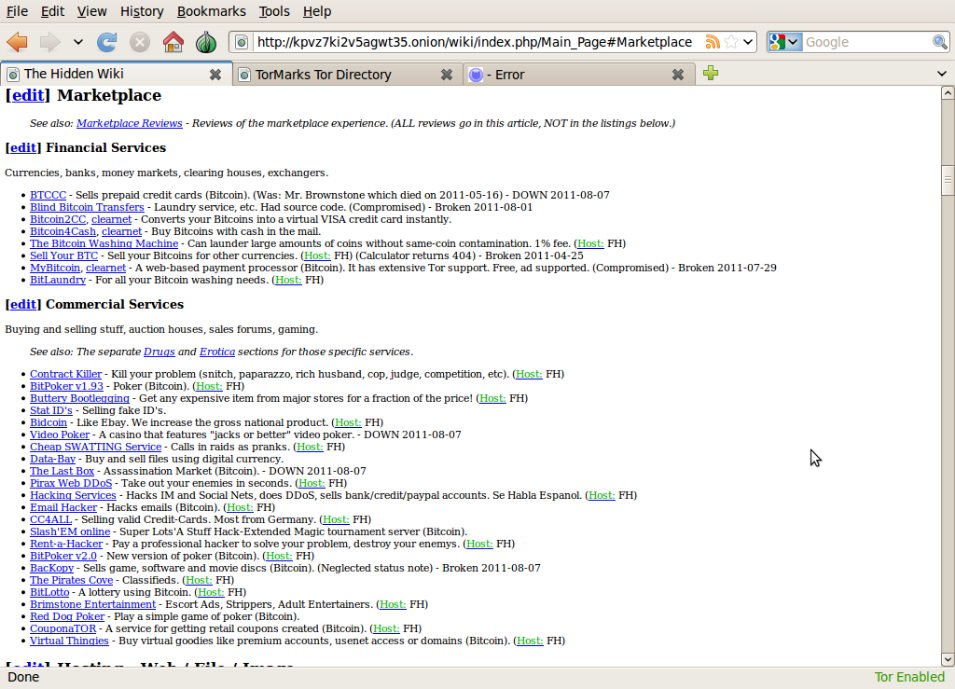
\includegraphics[width=0.9\textwidth]{resources/hiddenservice01.png}
                \caption{Ejemplo de \emph{Hidden wiki}, como vemos, una interfaz gráfica de hipervínculo burda y poco intuitiva, 
                    desde el punto de vista del desarrollo de \emph{Frontend} moderno}
                \label{}
            \end{figure}

    \subsection{Criptomonedas en Tor} 

        Un elemento altamente utilizado en la red Tor, no podía ser otro que las criptomonedas: <<monedas>> digitales --o 
        divisas-- para intercambios financieros en entornos informático, a menudo sin necesidad de intermediario ni servicio 
        centralizado. Debido precisamente a esta característica, la capacidad de dotar de privacidad y anonimato a una 
        transacción económica no sólo es útil, sino necesario a la hora de mantener nuestra identidad oculta en la red.
        De nada serviría, mantener nuestro anonimato en Internet si utilizamos nuestra cuenta bancaría para comprar 
        determinados artículos, delatándonos. Por ello las criptomonedas son la moneda de cambio preferida en esta red. 
        Normalmente, se hace referencia únicamente a \emph{Bitcoin}, por ser la más conocida; pero el mundo de las 
        criptomonedas es tan amplio, tanto a nivel financiero como matemático y criptográfico --e informático evidentemente-- 
        que no podemos reducirlo a la existencia a sólo una de ellas. Sería como hablar de microprocesadores y sólo detenernos 
        en Intel, por ser el más conocido y extendido.

        Aunque no es competencia directa del tema tratado, pues sólo es una característica utilizada dentro de la red, sí es 
        necesario indicar varios elementos clave. Sin tratar en profundidad, pues eso haría necesario la formación de un 
        trabajo tan --o más-- extenso que éste.
        
        El bitcoin apareció en 2009 para revolucionar el sistema de transacciones monetarias. La primera transferencia con 
        criptomoneda fue creada por \emph{Satoshi Nakamoto}, un alias del que aún se desconoce la identidad real.Esta moneda 
        digital nació con la intención de ser un intercambiador de valor digital que no dependiera de una entidad central 
        de emisión de capital; es decir, sin intermediarios que puedan registrar movimientos ni transacciones. Así como estar 
        <<a salvo>> del sistema económico y ser, en teoría, inmune a crisis económicas, inflación, etc. 
        
        \begin{figure}[htp]
            \centering
            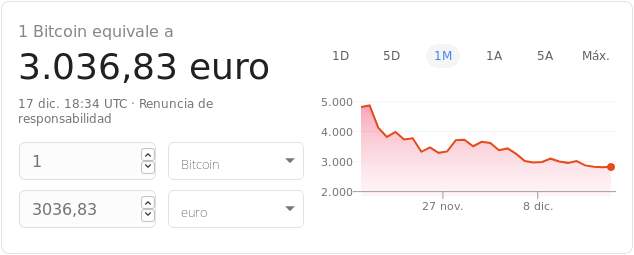
\includegraphics[width=0.9\textwidth]{resources/criptomonedas00.png}
            \caption{Equivalente en divisas de 1 Bitcoin en Euro (3.036,63) en la actualidad. Fuente: conversor de Google Inc.}
            \label{}
        \end{figure}
        
        Como la propia red Tor es \emph{un arma de doble filo}, dotando de capacidad financiera privada y anónima a los 
        usuarios. Esto atrae tanto a personas con necesidad real y moral de estas transacciones (por ejemplo, disidentes 
        políticos) como delincuentes que operan en Internet. A raíz del éxito de Bitcoin, en los últimos años no han dejado 
        de aparecer nuevas criptomonedas con diferentes capacidades y características para hacer frente al conocido Bitcoin.
        
        \begin{figure}[htp]
            \centering
            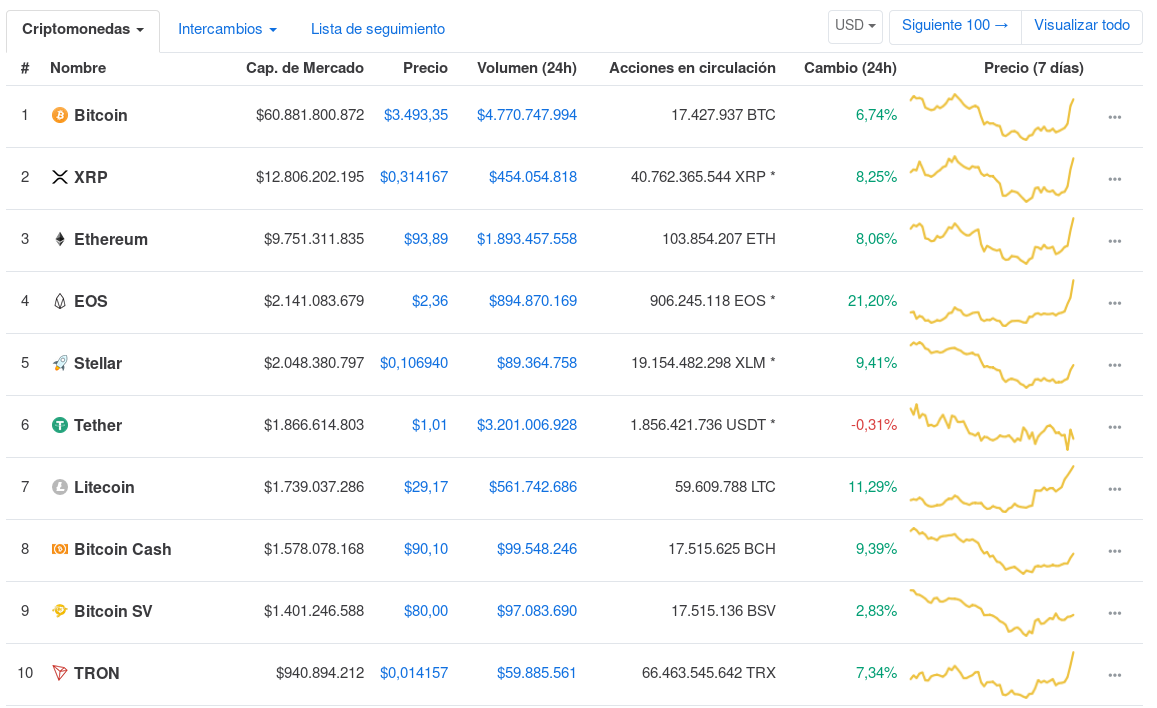
\includegraphics[width=0.9\textwidth]{resources/criptomonedas01.png}
            \caption{Principales Criptomonedas por capitalización de mercado. Fuente: \underline{https://coinmarketcap.com/es/}}
            \label{}
        \end{figure}
        
        De entre ella podemos destacar: \emph{XRP}, \emph{Ethereum}, \emph{Litecoin}, \emph{TRON}, \emph{NEO}, \emph{Qtum}, 
        \emph{DeepOnion}, etc. Pero la más destacable, tanto por su finalidad como por el contexto en el que nos hayamos, no 
        puede ser otra que \emph{\textbf{TorCoin}}: moneda virtual en gestación, desarrollada como modelo de software libre y 
        basada en el propio protocolo de Bitcoin.
        
        Ha sido desarrollada en sus inicios por investigadores de la \emph{Universidad de Yale}, donde destacamos las 
        personalidades de \emph{Miles Richardson}, \emph{Mainak Ghosh} y \emph{Bryan Ford} junto a \emph{Rob Jansen}, 
        líder de la \emph{Comunidad Tor} en 2014, año de lanzamiento de la criptomoneda. A pesar de, técnica y funcionalmente 
        tratarse de una divisa digital --podríamos decir-- común, traía consigo una motivación e innovación que le asegura 
        futuro dentro de la red Tor: 
        
        Puesto que Tor requiere de nodos, y estos nodos requieren de voluntarios que mantengan estos nodos en servidores con 
        capacidad suficiente (cuanto más nodos más seguridad habrá, pues más se incrementará exponencialmente la dificultad 
        de penetrar la seguridad de esta red e identificar un usuario concreto) era necesario --en el contexto histórico de 
        los años 2013-2014, en los que el total de nodos de Tor bajaron paulatinamente-- incentivar a los voluntarios a ceder 
        espacio de procesamiento y servidores para poder así mantener esta red en pleno funcionamiento. Con el nacimiento de 
        TorCoin pretendían entonces incentivar a estos voluntarios pero, ¿cómo?: permitiendo y facilitando que los dueños de 
        estos servidores pudiesen utilizar capacidad de procesamiento otorgado además por la red, para minar\footnote{
        \emph{La minería de criptomonedas es el proceso mediante el que se generan los bloques de la cadena de bloques, lo 
        que constituye la manera de procesar y verificar las transacciones. Agregar un bloque a la cadena de bloques es 
        difícil, requiriéndose tiempo y potencia de procesamiento para conseguirlo. Entonces, ¿qué incentivo tendría nadie 
        para realizar el esfuerzo de generar un bloque? La respuesta es que la persona que gestiona la producción de un 
        bloque consigue una recompensa. Dicha recompensa es doble: Por una parte, el productor consigue una gratificación 
        de un número determinado de por ejemplo, bitcoins, acordado por la red (actualmente esta gratificación es de 50 
        bitcoins; este valor disminuirá a la mitad cada 210.000 bloques). Por otra parte, cualquier comisión que pudiera 
        estar presente en las transacciones que se incluyan en el bloque, podrá ser reclamada por el productor de dicho 
        bloque.} Categoría:Minería, Wikipedia} esta criptomoneda (y así permitir enriquecerse económicamente, en mayor o 
        menor medida, a los voluntarios). Es decir, cualquier persona u organización que contribuya a la red con nodos de 
        Tor,obtendrá beneficios en TorCoins.
        
        Los impulsores de esta iniciativa, afirman que esta innovación incentivará a muchos más usuarios a correr los nodos 
        de Tor, resolviendo así el problema de ancho de banda y el crecimiento de la red, no sólo manteniendo el anonimato
        de la red Tor actual, sino inclusive perfeccionándolo y aumentando la comunidad.
    

\section{Tor sobre GNU/Linux}

    % TODO

\section{Hidden Service sobre GNU/Linux}

    % TODO

\section{Mitos y realidades de la red Tor}

    \subsection{¿Es tan segura la red Tor? Amenazas a la seguridad de Tor}

        A continuación analizaremos y enumeramos algunas amenazas a la seguridad de esta red y a sus usuarios.

    \subsubsection{Seguridad del sistema}

        El primer punto parece elemental, pero es necesario indicarlo. A pesar de que Tor nos ofrece un elevado 
        nivel de seguridad y anonimato, si nuestro sistema operativo, nuestra máquina, es vulnerable todo nuestro 
        sistema podrá estar comprometido.

        \begin{center}\emph{Publican un exploit utilizado para identificar a los usuarios de la red Tor en Microsoft Windows:}\end{center}
        \begin{center}\emph{https://www.redeszone.net/2016/11/30/publican-exploit-utilizado-identificar-los-usuarios-la-red-tor/?utm\_source\=related\_posts\&utm\_medium\=widget}\end{center}

        Esto también es aplicable al uso y mantenimiento de un Hidden Service. Si nuestro servidor no tiene la 
        suficiente seguridad, se encuentra desactualizado o es vulnerable a ataques de cualquier tipo (\emph{SQL Injection}, 
        \emph{XSS}, \emph{Exploits}, \emph{0-Days}) este será vulnerable como cualquier servidor. Por lo que NO es 
        suficiente utilizar Tor para garantizar la seguridad del sistema.

    \subsubsection{Aplicaciones inseguras}

        Al igual que el sistema, si utilizamos aplicaciones (principalmente las que tienen acceso a Tor) desactualizadas 
        o con diferentes vulnerabilidades podremos en peligro la seguridad de la navegación. Por ejemplo, la utilización 
        de un navegador desactualizado.

    \subsubsection{Configuración carente de seguridad}

        De igual forma, por muy seguro que sea nuestro sistema, si no tenemos una buena configuración de las aplicaciones 
        torificadas o el propio navegador podríamos identificarnos y poner nuestra seguridad en peligro.

        Por ejemplo, si nuestro navegador permite la ejecución de código \emph{Javascript} (el cual se descarga y ejecuta 
        en el equipo \emph{CLIENTE}) podríamos encontrarnos con un código malintencionado y comprometer nuestra seguridad.
        También es recomendable deshabilitar de nuestro navegador el protocolo \emph{WebRTC}, que puede identificarnos de 
        forma única evadiendo el anonimato de Tor o \emph{VPN}.

        Para minimizar este peligro es altamente recomendable la utilización del navegador propio de \emph{Tor Project}. 
        El cual viene preconfigurado para garantizar la seguridad de sus usuarios.

    \subsubsection{Control del nodo de entrada}
        
        Aunque en este proyecto no hemos ahondado en la técnica para construir nodos, ya sean de entrada, de salida o 
        intermedios, es necesario indicar que es posible hacerlo. Quizás el más difícil por su elevado control y seguridad 
        es montar (y que Tor acepte) un nodo de entrada.
        
        ¿Por qué? Porque este nodo, aún no viendo el contenido de los paquetes ya que van cifrados por capas, si ve la 
        dirección IP origen del cliente. El que controle un nodo de entrada controla la identidad de los usuarios de Tor 
        que utilizan este nodo para acceder a esta red. Por ello mismo es tan difícil y hay que cumplir tantos requisitos 
        para que Tor acepte nuestro nodo como nodo de entrada.
        
        Pero como sabemos, no existe la seguridad 100\%. Si alguien consigue tomar el control de un nodo de entrada, 
        controlará la identidad de los usuarios. ¿Y cómo alguien puede tomar el control de éste? Puede montarlo él mismo 
        y conseguir cumplir los requisitos, puede aprovechar alguna vulnerabilidad de uno de estos servidores para hacerse 
        con su control, puede obtener con cualquier técnica las credenciales al mismo, etc.

        \begin{figure}[htp]
            \centering
            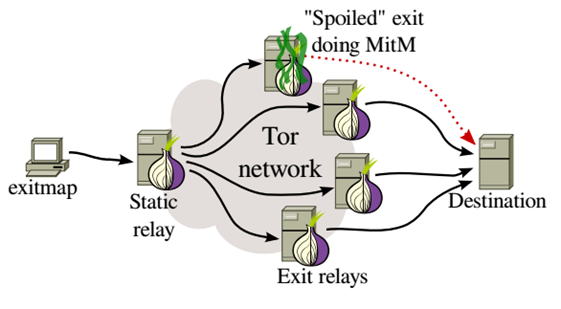
\includegraphics[width=0.9\textwidth]{resources/torspoiled.png}
            \caption{Nodo de Tor <<spoiled>> realizando ataques \emph{MitM} ó \emph{Man in the Middle}}
            \label{}
        \end{figure}
            
        \subsubsection{Control del nodo de salida}

            A diferencia que el nodo de entrada, montar un nodo de salida es relativamente fácil de conseguir. Quien 
            controla el nodo de salida controla el tráfico \emph{NO CIFRADO} de la red Tor. No sabrán de dónde viene 
            ese tráfico, eso sí, pero podrán controlarlo así.

            Los requisitos para ser aceptado como nodo de salida son factibles para cualquiera que se lo proponga: un 
            servidor lo suficientemente potente para controlar tráfico (como cualquier proxy, firewall, servidor web, 
            etc) y un suficiente ancho de banda. Simplemente con estos requisitos y un tiempo de prueba (puede ser de 
            varias horas incluso) para que Tor lo clasifique como nodo ‘de confianza’ será suficiente.
           
            \begin{figure}[htp]
                \centering
                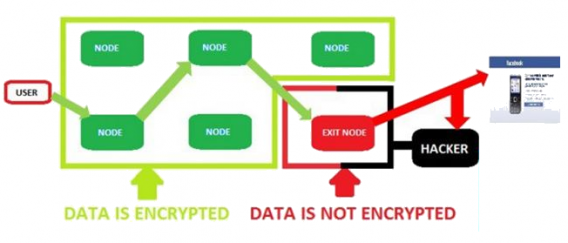
\includegraphics[width=0.7\textwidth]{resources/torspoiled2.png}
                \caption{Gráfico sencillo que representa el peligro del nodo de salida}
                \label{}
            \end{figure}

            En el blog de seguridad informática en el que el autor del presente documento ha sido miembro y cofundador, 
            \emph{Follow the White Rabbit} (\emph{fwhibbit.es}) se llevó a cabo una \emph{investigación}\footnote{Esta 
            investigación puede verse en el enlace \\ 
            \underline{https://www.fwhibbit.es/24-horas-en-la-vida-de-un-nodo-de-salida-de-tor} del blog} práctica sobre 
            el control de salida de un nodo de Tor, con el objetivo de experimentar y evaluar así los riesgos expuestos 
            en este punto. Como resumen de la investigación realizada y conclusión, se alcanzó en muy pocos días la 
            función de \emph{nodo de salida}, dando pie a la monitorización total del mismo, llegando incluso a obtener 
            credenciales de sitios inseguros (credenciales enviadas sin protocolos seguros, por ejemplo \emph{https}).

            \begin{figure}[htp]
                \centering
                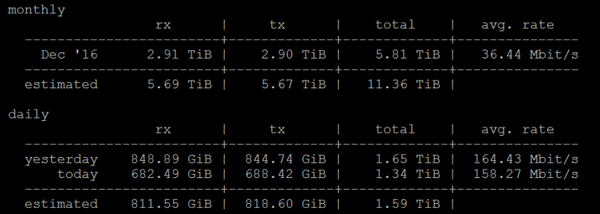
\includegraphics[width=0.9\textwidth]{resources/nodosalida00.png}
                \caption{<<Al final nuestro nodo Tor ha terminado moviendo mas de un 1.5 Terabyte de tráfico diario>>}
                \label{}
            \end{figure}

            De esta forma es fácil conocer qué están haciendo con el nodo de salida. Igualmente existen muchas formas 
            diferentes de obtener el control de un nodo de salida.

            Por supuesto en el momento que una persona tome el control de un nodo de salida y uno de entrada, comprometerá 
            completamente la seguridad de todos los usuarios que los utilicen.

        \subsubsection{Fugas de información}
        
            Aún manteniendo una seguridad técnica elevada, siempre podemos estar expuestos a fugas de información, a 
            menudo por despistes o inconsciencia de los usuarios. Por ejemplo, utilizar una aplicación sin utilizar Tor 
            y delatando nuestra identidad segundos antes de volver a acceder con Tor. Por ejemplo un hacker que lance un 
            exploit a través de Tor a un equipo, segundos después de haber realizado un escaneo de puertos sin Tor.

            Otro ejemplo bastante común es el acceso a sitios habiendo iniciado sesión en un perfil personal simultáneamente.
            Como acceder a Facebook mediante Tor y a su vez buscar anonimato.

        \subsubsection{Ingeniería social}
       
            Y, como siemp\textbf{re, \emph{el eslabón más débil de la cadena de la seguridad informática es el ser humano}}. 
            Podrían delatar nuestra identidad mediante técnicas de ingeniería social. Por ejemplo, un usuario de un chat que 
            obtenga nuestros datos personales utilizando la persuasión. 

        \subsection{Autodefensa y securización}

            Conociendo algunas de las amenazas, es necesario tomar medidas acorde a las mismas. Algunos consejos y medidas 
            a tomar son:

            \begin{enumerate}
                \item \emph{Utilizar el sentido común}. Si buscamos anonimato, no conectarnos a nuestros perfiles 
                personales que nos identifican. Ni decir nuestro nombre en los foros que visitamos. Ni utilizar nuestro 
                correo personal para acceder a diferentes sitios.
                \item \emph{Conocer Tor}. No todas las aplicaciones que iniciamos contarán con acceso a Tor. Deberemos 
                configurar cada aplicación para obtener esta característica. Por lo tanto, no pensemos que al instalar 
                Tor Browser ya estamos seguros y podemos descargar películas por Torrent sin peligro alguno.
                \item \emph{Evitar software privativo}, como Microsoft Windows, así como software desactualizado o 
                \emph{poco fiable}.
                \item \emph{Nuestro navegador debe ser una puerta de salida, pero no de entrada}. Bloquear códigos que 
                intenten ser ejecutados en nuestra máquina, como \emph{Javascript} o \emph{Flash}.
            \end{enumerate}

\section{Aspectos legales}

    \subsection{Legislación}

        Como venimos diciendo en repetidas ocasiones el presente documento, debido a que Tor ha sido considerado como 
        refugio de criminalidad se concibe como una importante amenaza para los gobiernos a nivel internacional. La 
        regulación legal en esta materia determinará las posiciones de distintos gobiernos en base a Internet, el uso y 
        derecho a la privacidad así como lo relacionado con el proceso criminal y penal en este contexto.

        Desde esta perspectiva podemos observar una complicada relación entre Tor, como concepto y algunos --si no la 
        mayoría-- de gobiernos. Además, hay que especificar un elemento esencial que supone un plus de dificultad a una 
        actuación y regulación conjunta en la  materia, la falta de formación de todos los agentes y personal en materia 
        tecnológica. De ahí radica la importancia de  los  países  que  utilizan la propia red Tor para la investigación 
        de la cibercriminalidad y aplicación de la ley,  aunque destacando la falta de regulación  y habiendo de  
        establecer los límites legales para no acabar vulnerando derechos. 

        Podemos destacar, pues, países como Holanda, Bélgica, Alemania, Noruega, Estados  Unidos y la propia España que 
        han posibilitado charlas de formación en Tor a sus policías y fuerzas de seguridad y orden, destacando, en  
        especial, el FBI en Estados Unidos, la Interpool y Europool en Europa y, concretamente la labor de la Policía 
        Nacional Española y la Guardia Civil en nuestro país. De manera que se concibe como un medio a través 
        del cual se aplica la ley a nivel nacional para la realización de las investigaciones criminales. Primordialmente 
        se  destacan tres actividades. Por un lado, se destaca la vigilancia online, es decir, posibilita la  
        navegación de los funcionarios por sitios  web y servicios no dejando rastro, evitando   
        así la obstaculización  de la investigación, \emph{Strings operations}\footnote{Operaciones encubiertas 
        realizadas por oficiales de la ley aprovechando el anonimato de la red.} y \emph{líneas de sugerencia anónima} 
        protegiendo la identidad digital del informador o denunciante.

        La simultaneidad de aplicación de la ley y uso de Tor supone cuestionarse qué límites se encuentran desde el 
        ámbito legal al utilizarse para recabar información, reunir evidencias así como en considerar los datos subidos 
        a la red Tor como información disponible públicamente. Esas limitaciones referidas, al estar previstas en cada 
        legislación nacional, presenta variaciones entre los países. En especial, destaca en la recopilación de pruebas 
        ya que al ser de carácter digital suponen importantes retos desde el punto de vista procesal. También se estudia 
        el tratamiento que reciben los datos de carácter personal, que se encuentran en las bases de datos que forman 
        parte de sus servicios ocultos.

        De manera que se parte de considerar a Tor como una herramienta que garantiza la libertad  virtual y permiteeludir
        la censura y restricciones impuestas en el ámbito electrónico. Por tanto, hay que destacar la importancia de la 
        privacidad ya que  es reconocido como derecho fundamental tanto en la Declaración Universal de los Derechos Humanos 
        como en los Código Penales y legislaciones nacionales. Por su relevancia, se pretende protegerla y garantizarla 
        en el entorno cibernético a través del desarrollo de herramientas como  Tor. Esto es debido a que se considera 
        que desde los propios gobiernos se pretende anteponer el orden público y seguridad colectiva a cualquier conducta 
        que consideren amenaza. Por tanto, este conflicto entre libertad virtual y seguridad requiere del desarrollo de 
        medidas y herramientas que, frente a las represiones y restricciones impuestas, garanticen el ejercicio de un 
        derecho fundamental. La sociedad demanda mayor libertad y privacidad ya que el nivel de control ejercido supera 
        los límites de lo que se considera necesario para garantizar la seguridad buscada. Como consecuencia de las 
        continuas regulaciones y leyes dirigidas a la creciente sanción de conductas y limitación de derechos, ciertos 
        sectores y miembros de la sociedad deciden acudir a estas medidas específicamente diseñadas para conseguir el 
        anonimato. 

    \subsection{Problemática legal}

        El derecho internacional en el ámbito tecnológico-informático juega un papel fundamental  en  este  escenario: 
        cuando un Estado interviene los servidores situados en el extranjero necesita de consentimiento concedido por 
        ese Estado --o de otros motivos de acuerdo a la normativa internacional--, entonces es cuando observamos la 
        problemática legal, en la que el uso de estas tecnologías y estas redes se hacen conflictivas con la jurisdicción: 
        cuando nos conectamos al servidor de Yandex\footnote{Conglomerado tecnológico equivalente al conocido \emph{Google} 
        en Rusia y alrededores.} nos estamos conectando a un equipo que se encuentra en alguna ciudad rusa, hipotéticamente 
        San Petesburgo. Si visualizamos contenido o realizamos acciones ilegales en uno u otro país, observamos un claro 
        conflicto entre ambas jurisdicciones y en el propio derecho internacional. Este conflicto se acentúa 
        considerablemente si hablamos de un acceso a la red Tor, que se distribuye entre nodos repartidos por el globo.

        La capacidad de superar cualquier frontera física y llegar a todas partes del mundo tiene esta grave consecuencia 
        ya que su omnipresencia se traduce en  importantes problemas de carácter legal dificultando su regulación y 
        penalidad (\emph{dificultad  probatoria}).

        También destaca el hecho de que se hayan retenido servidores cuyos usuarios son personas no relacionadas con la 
        investigación en curso. De manera, que habría una clara vulneración del derecho a la libertad que podría ser 
        llamada virtual, en cuanto a acceder libremente a donde el usuario quiera sin que se le restrinjan accesos ni 
        se les intente acusar de poseer servidores unidos con la actividad criminal.

        \emph{"Se dice que el castigo depende de la legislación del Estado en el territorio del cual se  encuentran  
        dichos  servidores  investigados. De  manera  que  se estaría haciendo referencia al principio de la 
        territorialidad, el cual con el mundo virtual parece  desvirtuarse  ya  que  la  realización  de  las  conductas  
        a  distancia  trasciende  de cualquier  territorio  físico,  pudiendo  iniciarse ,  realizarse  y  consumirse  en 
        lugar es totalmente diferente s .  Esto  plantea  disparidad  de  criterios  por  p arte  de  la  doctrina y 
        soluciones  dispares ante  este  fenómeno  complejo. Por tanto, se está hablando del desconocimiento de dónde y 
        quién comete los delitos por lo  cual  supone  no  poder  actuar  en  su  contra.  Por  ello , se  entiende  que  
        no  se  puede conocer  el  ámbito  de  actuación  en  base  a  la  jurisdicción  sobre  el  territorio  donde  
        se tiene competencia , mientras no se conozca el lugar donde están los servidores físicos que  garantizan  el  
        funcionamiento  de  estas  webs. Es  aquí  donde  se  aplicaría  la legislación estatal correspondiente.
        Por otra parte, e s interesante destacar si el usuario, a efectos legales, puede ser castigado en  España por  
        el  uso  de  mecanismos  de  cifrado en  las  comunicaciones mantenidas  en  la  red . La diversa  legislación  
        nacional  sí permite  el  uso  de  del  cifrado en  la  navegación .  Partiendo  de  la  propia  Constitución  
        Española,  una  interpretación amplia  d e  su  art.  18.3  garantiza  el  secreto  de  las  comunicaciones  
        puesto  que  se 38 entiende, en relación al art. 24.2 de la misma, que la existencia de una ley que limitara 
        el uso del cifrado confrontaría con el derecho a no declarar contra uno mismo ya que supondría una especie de 
        obligación de revelar los medios que utiliza el usuario. Ello se  refuerza  con  el art. 36.1 de  la  Ley  32/2003,  
        de  3  de  noviembre,  General  de telecomunicaciones,  conocido  comúnmente  como  LGT , cualquier  tipo  de 
        información transmitida   media nte   redes   de   comunicaciones   de   carácter electrónico pueden protegerse  
        a  través  de  los  procedimientos  de  cifrado (Maeztu, Del derecho y las normas, 2013)."}
        \begin{flushright}Extracto de \emph{LA RED TOR: UN ANÁLISIS DESDE EL PUNTO DE VISTA TÉCNICO, DE SUS CONSECUENCIAS 
            PRÁCTICAS Y ASPECTOS LEGALES.}\end{flushright}
        \begin{flushright}Clara Esteller Vidal\end{flushright}
        Pero, \textbf{supuesto distinto y donde se presentan complicaciones a nivel legal sería en relación a la instalación 
        y administración de un nodo Tor}. Respecto  a  este  supuesto  cabe  destacar la  definición  dada  desde  el  
        punto  de  vista jurídico  (tan to  la  LGT  como  el  Real  Decreto 899/2009) como  un  operador,  cuya 
        definición se prevé en los mismos y se entiende que los nodos caben dentro de esta categoría de operador al 
        tener el equipo informático encendido y operativo y estar haciendo la función de enturamiento de tráfico. De 
        esta manera, las personas que ad ministran públicamente un nodo se les considera como operadores.

        Las investigaciones jurídicas están limitadas a su vez por leyes de protección de datos personales, como siempre 
        que equipos infomáticos que utilizan estas informaciones son analizados en estos términos. España y la Unión 
        Europea mantienen una fuerte protección a estos (especialmente LOPD\footnote{Ley Orgánica de Protección de Datos} 
        y GDPR\footnote{General Data Protection Regulation - Regulación General de Protección de Datos}), lo que añade a 
        la problemática los conflictos político-judiciales propios de estos contextos y leyes: diferentes normativas, 
        diferencias a la hora de discernir qué es un dato de carácter personal y qué no, discrepancias en la graduación 
        de estos, etc.

        Como podemos ver, Tor supone un añadido de dificultad y problemática a los conflictos político-judiciales y 
        del derecho internacional que ya presentaban Internet, incrementándolo exponencialmente --podríamos decir 
        metafóricamente que \emph{estos problemas se elevan al número de nodos conectados}--. Por lo que la solución a 
        estos problemas debería pasar primero por la resolución de tantísima problemática general para, después resolver 
        --seguimos hablando en derecho-- el caso concreto de Tor.

\section{Conclusiones}

    Para finalizar el proyecto dedicado a esta controvertida red, podemos concluir en que dar a Tor un significado delictivo 
    ontológico es fruto de la ignoracia en el sector y la técnica. \textbf{Tor es una tecnología}, que emplea diversas 
    técnicas criptográficas, computacionales, redes y nodos distribuidos para realizar un intercambio de información 
    privado y anónimo. Como toda herramienta, sea física o digital, puede ser utilizado de diversas maneras; \emph{un 
    cuchillo puede ser utilizado como utensilio de cocina y como arma blanca}, por lo que es absurdo <<demonizar>> una 
    herramienta como un cuchillo así como una herramienta como es Tor.

    Como hemos podido vislumbrar durante la investigación, la red Tor no está extenta de mitos y leyendas que oscurecen a 
    menudo su estudio y su uso. En parte motivado por diferentes gobiernos que ante las dificultades legislativas que la 
    envuelven y la capacidad de evitar censura prefieren hacer políticas que eviten que más usuarios accedan a estas redes. 
    Así como la cultura popular ha catalogado --exagerando-- de inmoral y peligrosa la red Tor (asumiendo por nuestra parte 
    la realidad del uso delictivo que a menudo se puede dar a esta red, aunque podemos decir que no es más que un mero 
    reflejo --más anónimo-- que la \emph{surface web} --Internet común--) también la ha envuelto en mitos referentes a su 
    infranqueable seguridad, cuando la realidad es que no existe sistema 100\% seguro en ningún aspecto físico (así como 
    la informática no se libra de esta regla); existen sistemas más o menos vulnerables, expuestos a más o menos riesgos, 
    pero nunca puede ser considerado un sistema seguro en su plenitud. Hemos pretendido, pues desmentir estas leyendas 
    populares para darle un enfoque técnico y realista a la red y lo que encierra.  

    Por ello y como finalización del proyecto podemos resumir el trabajo de investigación en la necesidad, para nuestra 
    seguridad en la red Tor (aplicable también a la surface web) aprender y utilizar el principal escudo y mejor medida 
    de seguridad: \textbf{el sentido común}.

% BIBLIOGRAFÍA Y REFERENCIAS
\newpage
\begin{thebibliography}{X}
    \bibitem{} Tor Project - Documentation - torproject.org/docs/documentation.html
    \bibitem{} Archwiki - Tor - wiki.archlinux.org/index.php/tor
    \bibitem{} CyberCamp 2016 - <<Cambiando el CuenTOR>> Francisco Rodríguez - INCIBE \& Manu Guerra - FCSE - youtube.com/watch?v=PYu9Zkwmhw0
    \bibitem{} Follow the White Rabbit - <<24 horas en la vida de un nodo de salida de Tor>> - fwhibbit.es/24-horas-en-la-vida-de-un-nodo-de-salida-de-tor
    \bibitem{} Follow the White Rabbit - <<El nodo que todo lo ve>>  - fwhibbit.es/el-nodo-que-todo-lo-ve
    \bibitem{} Follow the White Rabbit - <<Creación de un Hidden Service de Tor>> por Francisco Javier Balón Aguilar - fwhibbit.es/creacion-de-un-hidden-service-de-tor
    \bibitem{} Follow the White Rabbit - <<Paranoicos I – VPN y Tor>> por Francisco Javier Balón Aguilar - fwhibbit.es/paranoicos-i-vpn-y-tor-2
    \bibitem{} I2P vs. Tor vs. VPN: Which Is More Secure? - makeuseof.com/tag/i2p-vs-tor-vs-vpn-secure/
    \bibitem{} Onion Routing - Computerphile - youtube.com/watch?v=QRYzre4bf7I
    \bibitem{} Encaminamiento cebolla - Wikipedia - es.wikipedia.org/wiki/Encaminamiento\_cebolla
    \bibitem{} Preguntas frecuentes - Bitcoin - bitcoin.org/es/faq
\end{thebibliography}

    
\end{document}
